\documentclass[conference]{IEEEtran}
\IEEEoverridecommandlockouts

% Local XeTeX/Tectonic builds only: IEEEtran's Times (ptm) is a pdfLaTeX font,
% so swap in the Times clone TeX Gyre Termes. Ignored under pdfLaTeX (Overleaf
% default), which is what the final submission should be compiled with.
\usepackage{iftex}
\ifXeTeX
  \usepackage{fontspec}
  \setmainfont{texgyretermes}[Extension=.otf, UprightFont=*-regular,
    BoldFont=*-bold, ItalicFont=*-italic, BoldItalicFont=*-bolditalic]
\fi

\usepackage{cite}
\usepackage{amsmath,amssymb,amsfonts}
\usepackage{graphicx}
\usepackage{booktabs}
\usepackage{multirow}
\usepackage{textcomp}
\usepackage{xcolor}
\usepackage{url}

\begin{document}

\title{Do Machine Learning Rankers Rescue Calendar-Month Seasonality? A Point-in-Time Walk-Forward Evaluation of Seasonal Stock Selection}

% ---- Replace with your details. IEEE conferences usually use double-blind
% ---- review: check the call for papers and anonymise this block if required.
\author{\IEEEauthorblockN{Vijayakumar Sitha Mohan}
\IEEEauthorblockA{\textit{Independent Researcher} \\
Weston, Florida, United States \\
smvk.2006@gmail.com}
}

\maketitle

\begin{abstract}
Calendar-month seasonality, the tendency of a stock to earn similar returns in the same calendar month across years, is a widely used retail and practitioner screening signal and a documented cross-sectional anomaly. Practitioner systems typically turn per-stock seasonal statistics into a hand-weighted z-score composite and validate it on the single calendar month for which the strategy was designed. We ask whether machine learning (ML) rankers improve on such a rule-based composite, and whether single-month validation overstates its value. We build a strictly point-in-time panel of 43{,}319 stock-month observations for 210 large-cap U.S. equities and evaluate rule-based and learned rankers (logistic regression, gradient-boosted decision trees, and a multilayer perceptron), each trained on an expanding window and retrained annually, over 252 out-of-sample months (2005--2025). In the November-only setting the production composite was designed for, it earns 3.45\% per month against 2.43\% for SPY. Over all months, however, no ranker beats an equal-weight benchmark of the same universe at conventional significance levels after 15\,bp transaction costs. The best performer, gradient boosting, adds 25\,bp per month (Newey--West $t=1.30$), and the seasonal filter on its own adds essentially nothing ($t=0.02$). Rank information coefficients are small (0.013--0.017), and the scores are poorly calibrated as probabilities. We conclude that single-month backtests of seasonal screens are vulnerable to calendar data snooping, and that standard ML rankers extract at most a weak, regime-dependent signal from these features.
\end{abstract}

\begin{IEEEkeywords}
algorithmic trading, return seasonality, machine learning, gradient boosting, walk-forward validation, backtest overfitting, computational finance
\end{IEEEkeywords}

% =====================================================================
\section{Introduction}

Calendar effects are among the oldest anomalies in empirical finance, from the January effect~\cite{rozeff1976} to the ``Sell in May'' pattern~\cite{bouman2002}. At the cross-sectional level, Heston and Sadka~\cite{heston2008} showed that stocks with high historical returns in a given calendar month tend to outperform in that same month in later years, and Keloharju \emph{et al.}~\cite{keloharju2016} documented that such return seasonalities appear across asset classes. These findings have been popularised in retail tools, which display per-stock ``seasonality'' tables (average return and win rate for each month) and invite traders to buy stocks entering historically strong months.

Turning such tables into a trading system involves many design decisions: thresholds that label a month ``Strong,'' minimum history requirements, hand-chosen weights for a composite score, and the choice of which calendar month to test. Each decision is a degree of freedom, and calendar effects in particular are known to be susceptible to data mining~\cite{sullivan2001}. In parallel, ML methods such as gradient-boosted trees and neural networks have been shown to improve cross-sectional return prediction from large characteristic sets~\cite{gu2020,krauss2017}. This raises a natural question for practitioners: \emph{can a learned ranker extract more from seasonal features than a hand-weighted composite, and does the answer survive an evaluation that does not cherry-pick the calendar month?}

This paper answers that question using a production seasonal-options screening pipeline as the object of study. Our contributions are as follows:
\begin{enumerate}
\item A strictly point-in-time evaluation protocol for seasonal stock selection that covers every calendar month, uses expanding-window ML training with annual retraining, and computes all features from data available at the prior month's close (Section~\ref{sec:method}).
\item A controlled comparison of a hand-weighted z-score composite against logistic regression, gradient-boosted decision trees (GBDT), and a multilayer perceptron (MLP) on identical features, universes, and costs, with momentum and equal-weight benchmarks (Section~\ref{sec:results}).
\item Evidence that a single-month backtest substantially overstates the value of the seasonal screen: November results that look strong do not generalise to the full calendar, and even the November filter result falls short of a multiple-testing-adjusted threshold (Section~\ref{sec:snooping}).
\item A calibration analysis showing that neither the composite score nor the ML probabilities map to monotonically increasing win rates, which argues against using them directly for position sizing (Section~\ref{sec:calibration}).
\end{enumerate}

% =====================================================================
\section{Related Work}

\textit{Return seasonality.} Heston and Sadka~\cite{heston2008} found that a stock's average return in the same calendar month over prior years predicts its relative return, an effect that persists for up to 20 years. Keloharju \emph{et al.}~\cite{keloharju2016} attributed seasonalities to recurring, seasonal variation in risk premia rather than to firm-specific events. Our feature set operationalises the practitioner version of this signal (same-month average return, win rate, and a binomial significance score) and adds the adjacent months.

\textit{Machine learning for cross-sectional returns.} Gu \emph{et al.}~\cite{gu2020} showed that tree ensembles and neural networks outperform linear models when predicting U.S. equity returns from a large set of firm characteristics. Krauss \emph{et al.}~\cite{krauss2017} and Fischer and Krauss~\cite{fischer2018} reported that GBDT, random forests, and LSTM networks generate statistical-arbitrage returns on S\&P~500 constituents. Unlike those studies, we restrict the input to a narrow, interpretable seasonal feature set, which is the setting most relevant to rule-based retail systems.

\textit{Backtest overfitting.} Lo and MacKinlay~\cite{lo1990} and White~\cite{white2000} formalised data-snooping bias. Sullivan \emph{et al.}~\cite{sullivan2001} showed that many calendar effects lose significance once the full universe of calendar rules that could have been tested is accounted for. Bailey and L\'opez de Prado~\cite{bailey2014} proposed the deflated Sharpe ratio, and Harvey \emph{et al.}~\cite{harvey2016} argued for higher significance thresholds in factor research. Survivorship bias in performance studies was analysed by Brown \emph{et al.}~\cite{brown1992}. We apply these lessons to a concrete practitioner system.

% =====================================================================
\section{Data and Methodology}\label{sec:method}

\begin{figure*}[t]
\centering
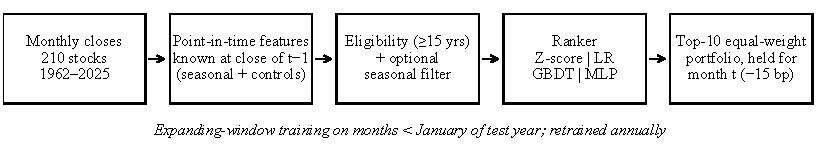
\includegraphics[width=\textwidth]{figures/pipeline.pdf}
\caption{Evaluation protocol. Every feature for target month $t$ is computed from data available at the close of month $t-1$. ML models are trained on all target months before January of the test year and retrained annually.}
\label{fig:pipeline}
\end{figure*}

\subsection{Universe and Data}
The universe consists of 210 U.S. large-cap stocks drawn from the S\&P~500 and Nasdaq-100, namely the constituents flagged by the production system's RSI-of-EMA scan on 6~October~2026, plus SPY as the market benchmark. Monthly split- and dividend-adjusted closing prices were obtained from Yahoo Finance and run from each stock's listing date (as early as 1962) through December 2025. Monthly simple returns are computed as $r_{i,t} = P_{i,t}/P_{i,t-1} - 1$.

Because the universe is defined by a 2026 condition, it is subject to survivorship and selection bias~\cite{brown1992}: firms that were delisted or left the indices before 2026 are absent. This biases the absolute returns of every strategy upwards. Consistent with this, the equal-weight (EW) universe beats SPY by 22\,bp per month (Table~\ref{tab:main}). We therefore treat EW as the primary benchmark. Every strategy is a top-10 selection from the same biased universe, so excess returns over EW measure the value of the ranking itself.

\subsection{Point-in-Time Features}
For stock $i$, target month $t$ (calendar month $m$, year $y$), let $\mathcal{R}_{i,m}^{<y}$ be the set of $i$'s returns in calendar month $m$ in years strictly before $y$. Following the production system, M2 denotes the target month, and M1 and M3 the preceding and following calendar months. We compute:
\begin{itemize}
\item M2 seasonal statistics: mean $\bar r_{i,m}$, win rate $w_{i,m}$ (share of positive returns), standard deviation, and history length $n_{i,m}=|\mathcal{R}_{i,m}^{<y}|$;
\item M1 and M3 mean returns, also over years $<y$;
\item cross-sectional excesses $w_{i,m}-\mathrm{med}_j\,w_{j,m}$ and $\bar r_{i,m}-\mathrm{med}_j\,\bar r_{j,m}$;
\item a significance score $-\log_{10}p_{i,m}$, where $p_{i,m}$ is the one-sided binomial $p$-value of observing $w_{i,m}n_{i,m}$ positive months under $H_0\!:\!p=0.5$;
\item non-seasonal controls: the prior-month return (short-term reversal), 12--1 momentum $P_{i,t-2}/P_{i,t-13}-1$~\cite{jegadeesh1993}, and trailing 12-month volatility.
\end{itemize}
A stock is \emph{eligible} at $t$ if $n_{i,m}\ge 15$. Over all months this gives 43{,}319 eligible stock-months (1995--2025), of which 37{,}259 fall in the 2005--2025 test period, with a median of 154 eligible names per month (range 108--178).

\subsection{Rule-Based Seasonal Filter and Composite}
A month is labelled \emph{Strong} if $\bar r\ge 1.5\%$ and $w\ge 55\%$, and \emph{Weak} if $\bar r\le -1.5\%$ and $w\le 45\%$ (requiring $n\ge5$). The production long filter keeps eligible names whose M2 is Strong, whose M1 and M3 are not Weak, and whose M2 win rate exceeds the universe median. Filtered names are ranked by
\begin{equation}
S_i \!=\! z(\Delta w_i) \!+\! z(\Delta \bar r_i) \!+\! \tfrac12\big[z(\bar r^{M1}_i) \!+\! z(\bar r^{M3}_i) \!+\! z(-\log_{10}p_i)\big],
\label{eq:zscore}
\end{equation}
where $z(\cdot)$ standardises a feature across the filtered set in that month. These are the production weights. Its RSI timing term is omitted because a historical RSI signal is not reconstructed here. At least one name passes the filter in all 252 test months (median 43).

\subsection{Machine Learning Rankers}
The learning task is binary classification. The label is $y_{i,t}=\mathbf{1}[r_{i,t} > \mathrm{med}_j\, r_{j,t}]$, i.e., whether the stock beats the cross-sectional median in the target month. To remove regime-level shifts, each of the 12 features is converted to its cross-sectional percentile rank within month $t$. We train three models with scikit-learn~\cite{pedregosa2011}:
\begin{itemize}
\item \textbf{LogReg}: $\ell_2$-regularised logistic regression ($C=0.5$) on standardised inputs;
\item \textbf{GBDT}: histogram-based gradient boosting~\cite{friedman2001,ke2017} with depth 3, learning rate 0.05, 200 iterations, at least 200 samples per leaf, and $\ell_2$ penalty 1.0;
\item \textbf{MLP}: two hidden layers (32, 16), weight decay $10^{-3}$, with early stopping.
\end{itemize}
Hyperparameters were fixed a priori to conservative values and not tuned on test data. For each test year $Y\in\{2005,\dots,2025\}$, each model is fit on all labelled stock-months with target date before January of $Y$ (the training panel starts in 1995) and scores every eligible stock in each month of $Y$. Each model ranks either the whole eligible universe or, in the ``+Filter'' variants, only filter-passing names.

\subsection{Portfolio Construction and Evaluation}
Each month, every strategy buys the 10 highest-ranked names in equal weight at the close of $t-1$ and holds them through month $t$, paying a flat 15\,bp round-trip cost. Benchmarks are SPY, the EW eligible universe, and a top-10 12--1 momentum portfolio. We report the mean monthly return, annualised return, volatility, Sharpe ratio, and maximum drawdown. For the excess return over EW we report the mean, a Newey--West~\cite{newey1987} $t$-statistic with three lags, and a 95\% moving-block bootstrap interval~\cite{kunsch1989} (block length 6, 5{,}000 resamples). Predictive accuracy is summarised by the monthly Spearman rank information coefficient (IC)~\cite{grinold2000} computed over the full eligible universe.

% =====================================================================
\section{Results}\label{sec:results}

\subsection{Full-Calendar Performance}

\begin{table*}[t]
\centering
\caption{Out-of-sample performance, all 252 months (Jan 2005 -- Dec 2025), top-10 equal-weight portfolios net of 15\,bp cost. Excess is versus the equal-weight (EW) eligible universe; $t_{\mathrm{NW}}$ is the Newey--West $t$-statistic; CI is the 95\% block-bootstrap interval. IC is the mean monthly Spearman rank IC over the eligible universe (its $t$-statistic in parentheses).}
\label{tab:main}
\footnotesize
\setlength{\tabcolsep}{4pt}
\resizebox{\textwidth}{!}{%
\begin{tabular}{lrrrrrrrrc}
\toprule
Strategy & Mean (\%/mo) & Ann. ret. (\%) & Ann. vol. (\%) & Sharpe & Max DD (\%) & Excess (\%/mo) & $t_{\mathrm{NW}}$ & 95\% CI & IC ($t$) \\
\midrule
SPY                 & 0.94 & 10.61 & 14.81 & 0.76 & $-50.8$ & $-0.22$ & $-2.28$ & $[-0.42,\,-0.02]$ & -- \\
EW universe         & 1.16 & 13.46 & 15.48 & \textbf{0.90} & $-47.2$ & -- & -- & -- & -- \\
12--1 Momentum      & 1.48 & 16.68 & 21.26 & 0.84 & $-46.9$ & 0.32 & 1.15 & $[-0.27,\,0.84]$ & $-0.005$ ($-0.35$) \\
\midrule
Seasonal filter (all) & 1.16 & 13.31 & 16.59 & 0.84 & $-49.2$ & 0.00 & 0.02 & $[-0.16,\,0.19]$ & -- \\
Z-score composite   & 1.34 & 15.38 & 18.30 & 0.88 & $-46.1$ & 0.18 & 1.00 & $[-0.16,\,0.57]$ & 0.017 (1.86) \\
\midrule
LogReg              & 1.34 & 14.32 & 22.66 & 0.71 & $-60.7$ & 0.18 & 0.87 & $[-0.19,\,0.59]$ & 0.014 (1.32) \\
GBDT                & 1.41 & 16.03 & 19.91 & 0.85 & $\mathbf{-43.5}$ & \textbf{0.25} & \textbf{1.30} & $[-0.07,\,0.67]$ & 0.013 (1.45) \\
MLP                 & 1.29 & 14.59 & 19.11 & 0.81 & $-46.6$ & 0.14 & 0.76 & $[-0.17,\,0.54]$ & 0.014 (1.78) \\
LogReg + Filter     & 1.26 & 13.78 & 21.10 & 0.72 & $-53.0$ & 0.10 & 0.52 & $[-0.26,\,0.55]$ & -- \\
GBDT + Filter       & 1.17 & 12.99 & 19.44 & 0.73 & $-44.2$ & 0.02 & 0.08 & $[-0.35,\,0.46]$ & -- \\
MLP + Filter        & 1.23 & 13.88 & 18.21 & 0.81 & $-40.5$ & 0.07 & 0.37 & $[-0.27,\,0.49]$ & -- \\
\bottomrule
\end{tabular}}
\end{table*}

Table~\ref{tab:main} reports the main results. Three findings stand out.

First, \emph{the seasonal filter by itself carries no information over the full calendar}. Holding every filter-passing name earns 1.16\% per month, identical to the EW universe, with higher volatility.

Second, \emph{ranking adds a modest but statistically insignificant return}. The z-score composite adds 18\,bp per month and GBDT 25\,bp, the largest of any strategy. Neither excess is significant ($t_{\mathrm{NW}}=1.00$ and $1.30$), and both bootstrap intervals contain zero. On a risk-adjusted basis, no strategy beats the EW universe's Sharpe ratio of 0.90: concentrating in 10 names raises volatility roughly in proportion to the added return. GBDT does post the shallowest drawdown ($-43.5\%$).

Third, \emph{restricting ML rankers to the seasonal filter hurts}. Every ``+Filter'' variant underperforms its unconstrained counterpart. GBDT drops from 25\,bp to 2\,bp, which suggests that the filter discards names the model would usefully rank.

Rank ICs are positive but small for all seasonal rankers (0.013--0.017), and none reaches $|t|\ge 2$. The z-score composite has the highest IC (0.017, $t=1.86$), so the hand-weighted linear combination is at least as informative as the learned models on these features. This is consistent with the low signal-to-noise ratio of monthly returns~\cite{gu2020}, in which flexible models gain little over simple ones on narrow feature sets.

\begin{figure}[t]
\centering
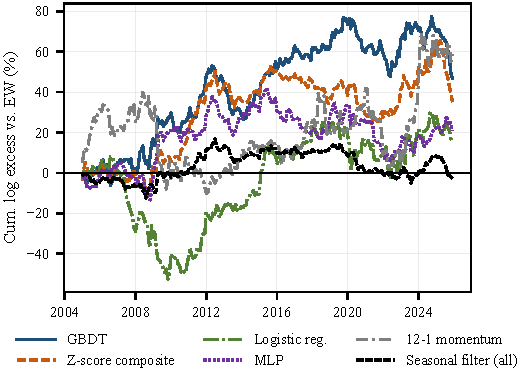
\includegraphics[width=\columnwidth]{figures/cum_excess.pdf}
\caption{Cumulative log excess return over the EW universe, 2005--2025. Excess returns are episodic: GBDT and the z-score composite gain mainly in 2009--2012 and give back part of that after 2020.}
\label{fig:cum}
\end{figure}

\subsection{Stability Across Time and Calendar Months}

Fig.~\ref{fig:cum} and Table~\ref{tab:sub} show that excess returns are concentrated in particular regimes. GBDT earns about 50\,bp per month over EW in 2005--2015 but $-15$\,bp in 2021--2025. Logistic regression shows the reverse pattern, with a deep drawdown in 2008--2010 followed by a strong 2011--2015. Momentum, the non-seasonal control, is the only strategy whose excess return rises in recent years. Fig.~\ref{fig:month} breaks excess returns down by calendar month. The composite's best months are January and February rather than November, and it loses about 1\% per month on average in July.

\begin{table}[t]
\centering
\caption{Mean monthly excess return over EW (\%) by sub-period.}
\label{tab:sub}
\begin{tabular}{lrrrr}
\toprule
Strategy & 2005--10 & 2011--15 & 2016--20 & 2021--25 \\
\midrule
Seasonal filter & 0.03 & 0.22 & $-0.18$ & $-0.07$ \\
Z-score         & 0.28 & 0.60 & $-0.32$ & 0.13 \\
LogReg          & $-0.56$ & 1.01 & 0.25 & 0.16 \\
GBDT            & 0.46 & 0.50 & 0.15 & $-0.15$ \\
MLP             & 0.35 & 0.30 & $-0.10$ & $-0.05$ \\
Momentum        & 0.17 & 0.11 & 0.44 & 0.60 \\
\bottomrule
\end{tabular}
\end{table}

\begin{figure}[t]
\centering
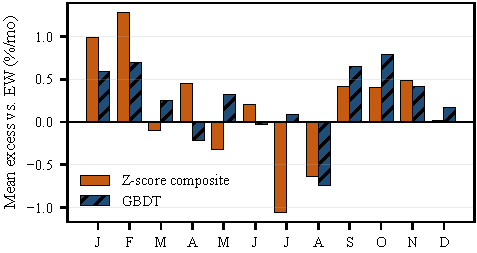
\includegraphics[width=\columnwidth]{figures/excess_by_month.pdf}
\caption{Mean monthly excess return over EW by calendar month (each bar averages 21 years).}
\label{fig:month}
\end{figure}

\subsection{Single-Month Evaluation and Calendar Data Snooping}\label{sec:snooping}

The production system was developed and backtested for a single configuration: scan in October and hold through November. Table~\ref{tab:nov} restricts the evaluation to the 21 Novembers. Our point-in-time implementation reproduces the production backtest's 3.45\% average November return for the z-score composite to two decimal places, which validates the implementation. Measured against SPY (2.43\%), the November result looks compelling. However:
\begin{itemize}
\item about half of the gap to SPY (52\,bp) is the universe effect: the EW universe itself earns 2.96\% in November;
\item in November the filter alone looks significant ($t_{\mathrm{NW}}=2.37$), but a researcher who could have chosen any of 12 calendar months faces a Bonferroni-adjusted two-sided 5\% threshold of $|t|\approx 2.87$, so the result does not survive a correction for the choice of month;
\item over the full calendar the same filter's excess return is $0.002\%$ per month ($t=0.02$).
\end{itemize}
This is the pattern that Sullivan \emph{et al.}~\cite{sullivan2001} warned about for aggregate calendar effects, here reproduced in a single practitioner system. The November configuration was the natural one to test given when the system was built, but that is precisely how an implicit search over calendar months enters a backtest.

\begin{table}[t]
\centering
\caption{November-only results (21 observations) compared with all months.}
\label{tab:nov}
\footnotesize
\setlength{\tabcolsep}{3pt}
\begin{tabular}{lrrrr}
\toprule
 & \multicolumn{2}{c}{November only} & \multicolumn{2}{c}{All months} \\
\cmidrule(lr){2-3}\cmidrule(lr){4-5}
Strategy & Mean & Excess ($t_{\mathrm{NW}}$) & Mean & Excess ($t_{\mathrm{NW}}$) \\
\midrule
SPY             & 2.43 & $-0.52$ ($-3.10$) & 0.94 & $-0.22$ ($-2.28$) \\
EW universe     & 2.96 & -- & 1.16 & -- \\
Seasonal filter & 3.28 & 0.32 (2.37) & 1.16 & 0.00 (0.02) \\
Z-score         & 3.45 & 0.49 (1.29) & 1.34 & 0.18 (1.00) \\
GBDT            & 3.37 & 0.41 (0.64) & 1.41 & 0.25 (1.30) \\
LogReg + Filter & 3.71 & 0.75 (1.79) & 1.26 & 0.10 (0.52) \\
\bottomrule
\end{tabular}
\end{table}

\subsection{Score Calibration}\label{sec:calibration}

Practitioner systems often map score tiers (e.g., A+/A/B/C) to position sizes, which implicitly assumes that higher scores mean a higher probability of a positive return. Fig.~\ref{fig:calib} pools all out-of-sample stock-months and plots the empirical probability of a positive return by score decile. The curves are flat, between 55\% and 60\%, with no monotone trend for any model. In the production system's own 21-year November backtest, the tier win rates (A+ 76.7\%, A 66.7\%, B 76.4\%, C 70.0\%) were likewise non-monotonic. The z-score composite's top decile does earn a higher mean return (1.76\% vs.\ 1.13\% for the bottom decile), so the score carries some information about the size of returns but little about their sign. Neither raw scores nor ML probabilities should be used as calibrated probabilities for sizing without post-hoc calibration, such as isotonic regression~\cite{zadrozny2002}, fitted out of sample.

\begin{figure}[t]
\centering
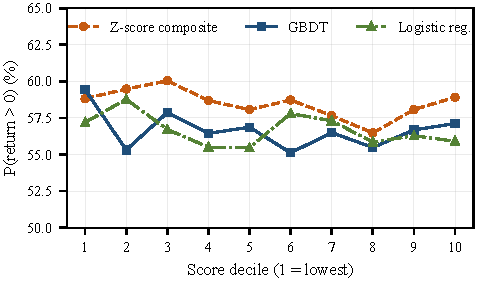
\includegraphics[width=\columnwidth]{figures/calibration.pdf}
\caption{Probability of a positive month-$t$ return by out-of-sample score decile (pooled 2005--2025).}
\label{fig:calib}
\end{figure}

\subsection{What the Linear Model Uses}
As a descriptive check, we fitted the logistic model once on all data (not used for trading). The largest coefficients were on adjacent-month seasonality (M1 negative, M3 positive), trailing volatility (positive), and the prior-month return (negative, consistent with short-term reversal). Coefficients on the target-month (M2) seasonal statistics that the rule-based system emphasises were close to zero. This suggests that whatever weak signal exists in these features comes from adjacent-month structure and risk-related controls, not from the same-month win rate.

% =====================================================================
\section{Discussion and Limitations}

\textit{Implications for practitioners.} A seasonal screen validated on one calendar month should be re-tested on all twelve before it is trusted, with the choice of month counted as a tested hypothesis. Replacing hand-chosen weights with an ML ranker is cheap and does no harm, but on this feature set it does not turn an insignificant edge into a significant one. Richer inputs are likely necessary, such as fundamentals, options-implied information, or the intraday timing signals used by the production system.

\textit{Limitations.} (i) Survivorship and selection bias in the universe inflate absolute returns. Relative comparisons are less affected but not immune, since the bias may interact with seasonal features. A point-in-time index-membership dataset such as CRSP would remove it. (ii) The universe is small (210 names), so the top-10 portfolios are concentrated and noisy. (iii) We evaluate only the seasonal component of the production system. Its RSI-of-EMA entry timing and its options-structuring stage (spread selection, liquidity and gamma-exposure checks) are not backtested, because historical option chains were not available. (iv) A flat 15\,bp cost understates the cost of option spreads. (v) Hyperparameters were fixed rather than tuned. Nested walk-forward tuning could help the ML models, but would itself be another source of selection bias.

% =====================================================================
\section{Conclusion}
We evaluated rule-based and machine-learning rankers built on calendar-month seasonal features over 252 strictly out-of-sample months. The production system's November backtest is reproducible but does not generalise. Over the full calendar, neither the seasonal filter nor any ranker beats an equal-weight benchmark of the same universe at conventional significance levels, although gradient boosting delivers the highest excess return and the shallowest drawdown. Scores are poorly calibrated as probabilities. Future work will replace the survivorship-biased universe with point-in-time index membership, add the RSI-based timing signal and options-implied features, and evaluate the options layer on historical chains.

\section*{Code Availability}
The experiment code, figure scripts, and result tables are available at \url{https://github.com/smvijaykumar/seasonal_options_system}.

\section*{Acknowledgment}
% IEEE policy requires disclosure of AI-generated content (text, figures,
% code) in the acknowledgments, naming the system and the sections it was
% used in. Edit this to reflect exactly how you used it.
The author used an AI assistant (Claude, Anthropic) to help develop the experiment code, generate the figures, and draft the manuscript text. The author reviewed, verified, and takes full responsibility for all content.

\bibliographystyle{IEEEtran}
\bibliography{references}

\end{document}
